\documentclass{standalone}
\usepackage{pgfplots}
\pgfplotsset{compat=1.17}
\usepackage{tikz}
\usepackage{amsmath}

\begin{document}

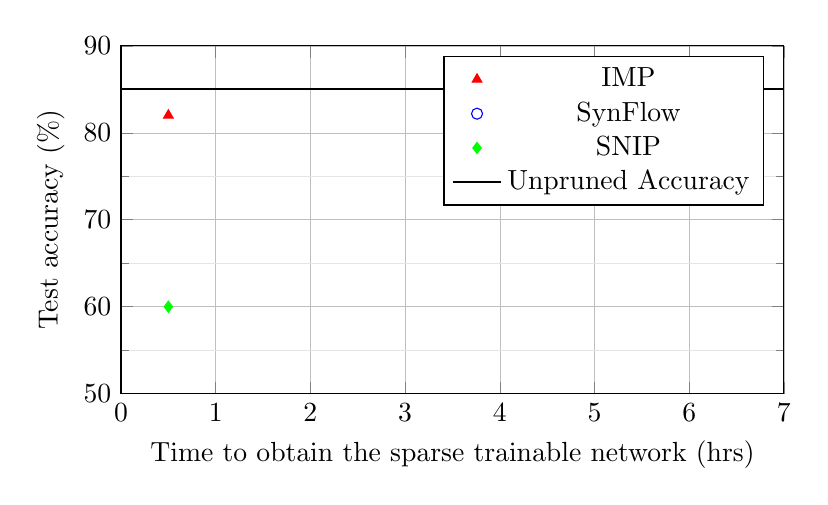
\begin{tikzpicture}
    \begin{axis}[
        width=10cm,
        height=6cm,
        xlabel={Time to obtain the sparse trainable network (hrs)},
        ylabel={Test accuracy (\%)},
        ymin=50, ymax=90,
        xmin=0, xmax=7,
        grid=both,
        minor y tick num=1,
        major grid style={line width=.2pt,draw=gray!50},
        minor grid style={line width=.1pt,draw=gray!20},
        legend pos=north east,
        legend style={draw=black, fill=white},
    ]
    
    % IMP data
    \addplot[
        only marks,
        mark=triangle*,
        mark options={fill=red},
        red
    ]
    coordinates {(0.5, 82)};
    
    % SynFlow data
    \addplot[
        only marks,
        mark=o,
        mark options={fill=blue},
        blue
    ]
    coordinates {(6, 79)};
    
    % SNIP data
    \addplot[
        only marks,
        mark=diamond*,
        mark options={fill=green},
        green
    ]
    coordinates {(0.5, 60)};
    
    % Unpruned Accuracy (line)
    \addplot[
        black,
        thick
    ]
    coordinates {(0, 85) (7, 85)};
    
    % Legend
    \legend{IMP, SynFlow, SNIP, Unpruned Accuracy}
    
    \end{axis}
\end{tikzpicture}

\end{document}